\documentclass[../BTOF_summary.tex]{subfiles}
 
\begin{document}


\section{Readout}

Foreseen is a readout with the TOFPET ASIC by PETsys Electronics.
However there have been no significant developments towards implementing the readout system for the \btofD .

The readout system consists of two main stages.
The first stage consists of an assembly of small analog boards as seen in \fig~\ref{fig:FEM128}, the FEB/A, which is part of the \textit{front end readout system}, holding the TOFPET ASIC, which converts the incoming signal into digital charge and timing information.
Two of these boards each carrying a single TOFPET ASIC connect to the FEB/I and FEB/S boards forming \textit{Front-End-Module 128} (FEM128), which is depicted in \fig~\ref{fig:FEM128}.

\begin{figure}[htbp]
    \centering
    \includegraphics*[width=.8\textwidth]{fig/FEB_A_I_S.png}
    \caption{Connection of the FEB/A to the FEB/S and FEB/I.}
    \label{fig:FEM128}
\end{figure}

The FEB/S is almost purely passive and acts as an adapter between the connection scheme of the sensors and the ASIC boards.
It however is also equipped with a temperature sensor to monitor the \sipms\ arrays which are supposed to be attached directly to the board.
The FEB/I however is equipped with a MAX 10 Altera FPGA to manage the temperature sensors and the communication between the ASICS and the readout.

A second version of the Front-End-Module, the FEM256, shown in \fig~\ref{fig:FEM256} equipped with four TOFPET ASIC's is also available for systems with a lower event rate.
It is only capable of delivering \SI{300}{kcps} which is more than enough for the up to \SI{40}{kHz} per channel average hit rate in the forward region of the detector.

\begin{figure}[htpb]
    \centering 
    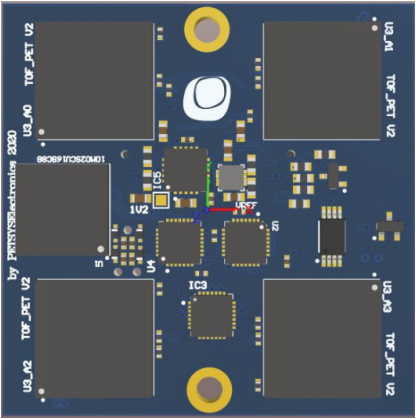
\includegraphics[height=6cm]{fig/FEM256_top.png}
    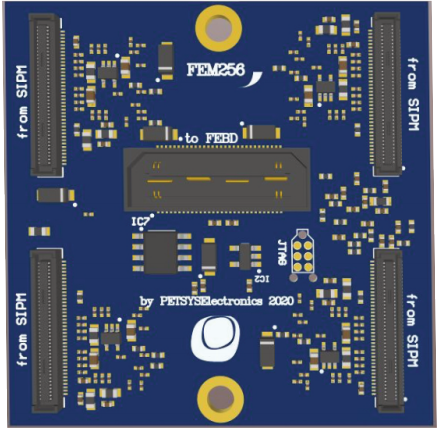
\includegraphics[height=6cm]{fig/FEM256_bottom.png}
    \caption{Front-End-Module 256 combining two FEB/A boards and the FEB/I into one single board capable of reading out 256 channels.}
    \label{fig:FEM256}
\end{figure}

The second stage is a digital board, the FEB/D, to which up to 8 Front-End-Modules ca be connected and which can be daisy-chained with other FEB/D boards for simple control.
If the number of channels grows beyond \num{1024} channels two additional boards, the \textit{DAQ Board} and the \textit{Clock\&trigger Module}, are required for the readout.

The c\&t module acts as the central connection hub for up to 16 FED/D boards and provides the system reference clock.
For the synchronization with external systems it can accept external clock and synchronization signals.
It connects to the DAQ Board the same way a FEB/D would.
The DAQ Board itself connects to a PC via a x4 PCI express port and can transmit \SI{200}{Mcps}.

The entire detector consists of \num{3840} channel.
Which necessitates the additional boards.
With an average hit rate per tile and channel of \SI{27}{kHz} a total event rate of \SI{104}{MHz} can be expected.

The first stage of the readout, the Front-End-Modules, needs to be positioned as close to the \sipms\ as possible, since they handle analogue signals.
For this reason they are placed on the \railboard s where the MMCX output connectors are position for the prototype.
The second stage, the FEB/D and subsequent boards can be setup up to \SI{3}{m} away by connecting long ribbon cables.
If the FEB/D is to be positioned on each \sm , for which there is more than enough space on the board, the xxx\todo[]{which component is this} components has to be changed, since it can not operate in large magnetic fields.
The DAQ and the C\&T boards are meant to be setup outside of the main detector.

Due to the small dimensions of the available space in the detector slot the boards for the detector need to be redesigned.

\end{document}